
\documentclass[a4paper,8pt]{article}

% Encoding.
\usepackage{hyperref}
\usepackage{geometry}
\usepackage[T2A]{fontenc}
\usepackage[utf8]{inputenc}
\usepackage[english,russian]{babel}

% Code insertion.
\usepackage[outputdir=build]{minted}

% Math functions.
\usepackage{amsmath}

% Image insertion.
\usepackage{svg}

% No line breaks.
\usepackage[none]{hyphenat}

\title{Задание 6: Технико-коммерческое предложение ``e-гриб''}
\author{
    \begin{tabular}[t]{c@{\extracolsep{8em}}c}
        Афанасов Артём     & Смирнов Александр \\
        &\\
        Струтовский Максим & Феодор Жилкин
    \end{tabular}
}

\date{\today}
\begin{document}

\maketitle
\tableofcontents
\newpage


\section{Информация о компании}

Наша компания ОАО ``Подрядчик-рус'' специализируется на запуске процессов интернет-магазинов, а также на отладке сопутствующих бизнес-процессов.

Мы представлены на рынке более 10 лет, успешно запустив более 200 проектов.
Мы обладаем опытом в более чем 50-ти нишах.



\subsection{Собственность}

    \begin{itemize}
        \item В собственности ОАО ``Подрядчик-рус'' находится 11 офисов в 5-ти городах России;
        \item 3 дата-центра;
        \item Общая численность сотрудников составляет более 3 тыс. человек;
        \item История исполнения предыдущих проектов.
    \end{itemize}



\subsection{Финансово-экономические показатели}



    \begin{itemize}
        \item Средняя выручка компании за последние три года составил 2 млрд. руб.;
        \item Средняя прибыль компании за последние три года составил 300 млн. руб.;
        \item Стоимость компании по последним оценкам составляет 5 млрд. руб.;
        \item Вся отчётность доступна на сайте налоговой службы.
    \end{itemize}


\subsection{Система менеджемента качества}


    \begin{itemize}
        \item Соответсвует ИСО 9001.
    \end{itemize}


\subsection{Процедуры управления проектами}


    \begin{itemize}
        \item Наши аналитики оценивают трудозатраты на выполнение проекта;
        \item Данный проект выполняется по системе оплаты фикс прайс;
        \item Разработка ведётся по методологии scrum.
    \end{itemize}



\subsection{Персонал}


    \begin{itemize}
        \item CEO (10 лет опыта в управлении компаниями с оборотом от 1 млрд. руб.);
        \item CTO (7 лет опыта на позиции CTO);
        \item Топ-менеждмент (от 5-ти лет опыта на подобной позиции): 10 чел.;
        \item Разрабочики (разный уровень, от juniour до seniour): 1500 чел.;
        \item Все остальные: 1488.
    \end{itemize}



\subsection{Квалификация}


    \begin{itemize}
        \item Вследствие огромного опыта компании мы обладаем сооствествующими квалификациями на всех рынках;
        \item В частности был успешно проработан и воплощён в жизнь проект по реализации кефирного гриба.
    \end{itemize}


\subsection{Заказчики}


    \begin{itemize}
        \item ЛАНИТ-ТЕРКОМ:
            \begin{itemize}
                \item Северо-Западный регион;
                \item Разработка компилятора РуСи;
                \item Андрей Николаевич Терехов, 88005553535;
            \end{itemize}
        \item matrasvam.com;
        \item ООО ``Slavic-Fit'';
        \item Google;
        \item Facebook;
        \item Alibaba Group;
        \item Яндекс.Гриб;
        \item ТНТ;
        \item Gerard Miller Inc.;
        \item ООО Продмастер.
    \end{itemize}


\section{Рамки проекта}


\subsection{Цели}


    \begin{itemize}
      \item Приложения под платформы:
          \begin{itemize}
              \item iOS;
              \item Android;
              \item Web;
              \item 3500 заказов ЧГ в день;
          \end{itemize}
      \item Произодство ЧГ:
          \begin{itemize}
              \item Ферма по производству ЧГ;
              \item 4000 ЧГ в день;
          \end{itemize}
      \item Организация доставки ЧГ до клиента:
          \begin{itemize}
              \item 3 склада в разных концах Санкт-Петербурга;
              \item Аутсорс доставки из складов;
          \end{itemize}
      \item Чистая прибыль 10 млн. руб. в месяц.
    \end{itemize}

\subsection{Ограничения}

    \begin{itemize}
        \item Финансы:
            \begin{itemize}
                \item 50 млн. руб.
            \end{itemize}
        \item Временные ограничения:
            \begin{itemize}
                \item 12 месяцев;
                \item Тренд на ЧГ;
                \item Конкуренция;
            \end{itemize}
        \item Ограничения по доставке:
            \begin{itemize}
                \item Санкт-Петербург.
            \end{itemize}
    \end{itemize}



\section{Описание решения проекта}


\subsection{Фазы проекта}

    \begin{itemize}
        \item Старт:
            \begin{itemize}
                \item Сформированы команды;
                \item Арендованы складские помещения;
            \end{itemize}

        \item Подготовка к запуску производства:
            \begin{itemize}
                \item Подготовлено оборудование для выращивания ЧГ;
                \item Закуплены расходные материалы (удобрения, субстракт, споры);
                \item Разработано бета-ПО;
            \end{itemize}


        \item Запуск производства:
            \begin{itemize}
            \item Налажено выращивание ЧГ;
            \item Налажена доставка до логистических центров;
            \item Финальная версия ПО;
            \item Налажена связь со службой поддержки;
            \item Маркетологи начали рекламную кампанию;
            \end{itemize}

        \item Начало продаж:
            \begin{itemize}
                \item Налажена доставка до потребителя.
            \end{itemize}

    \end{itemize}


\subsection{Диаграмма Ганта}

    \begin{itemize}
        \item Диаграмма Ганта изображена на Рис. 2 (можно приближать);
    \end{itemize}


    \begin{figure}[h]
        \centering
        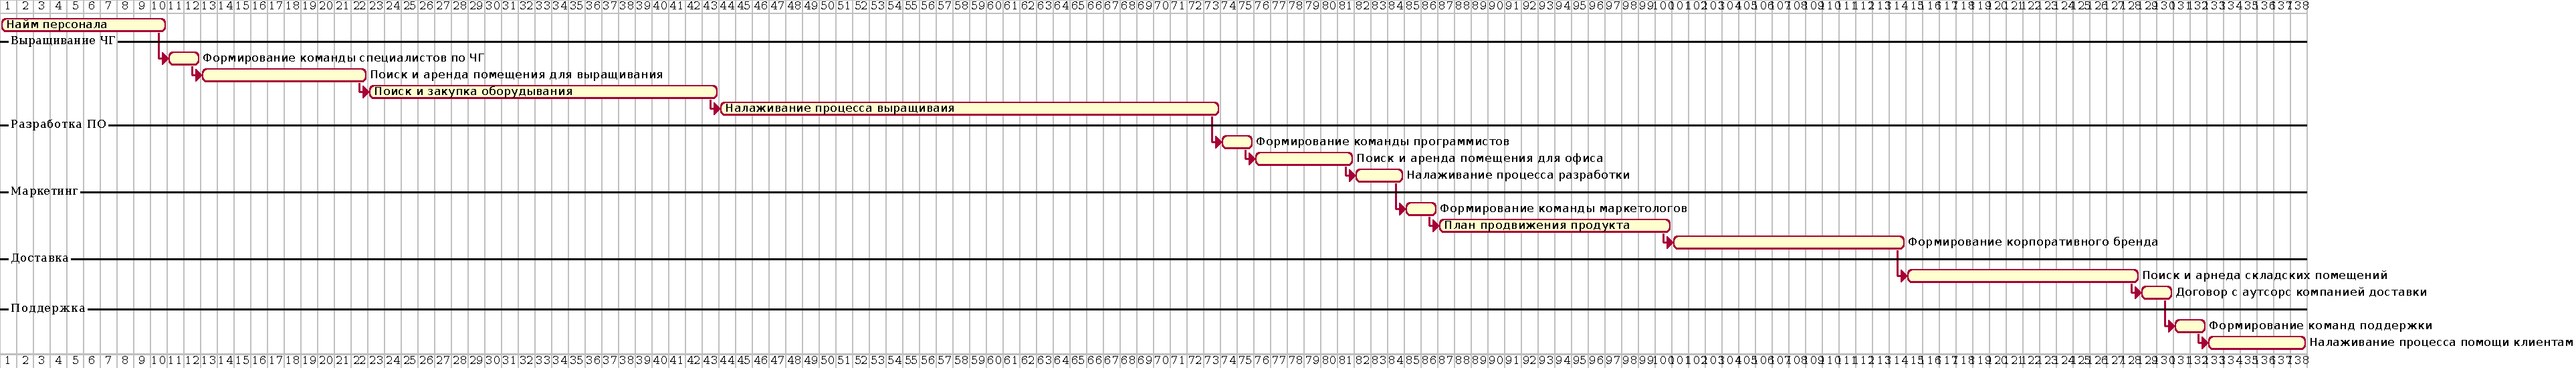
\includegraphics[width=1\textwidth]{./pics/gantt.pdf}
        \caption{gantt}
    \end{figure}




\section{Процедуры управления проектом}



\subsection{Типы отчётов}

    \begin{itemize}
        \item Ретроспетивы;
        \item Demo каждую неделю;
        \item Daily митинги;
        \item Финансовые отчёты;
        \item Отчёты с фермы;
        \item Отчёты от техподдержки;
    \end{itemize}


\subsection{Процедуры управления изменениями}

    \begin{itemize}
        \item Непрерывное взаимодействие с заказчиком
        \item Формирование требований для исполнителей
    \end{itemize}

\subsection{Процедуры анализа хода проекта}

    \begin{itemize}
        \item Спринты по 2 недели
        \item Финансовые отчёты каждый месяц
    \end{itemize}

\subsection{Методы планирования}

    \begin{itemize}
        \item Методология Kanban
        \item Ежедневные standup встречи по утрам
    \end{itemize}





\subsection{Участники коммуникации}

    \begin{itemize}
    \item Люди:
        \begin{itemize}
            \item Управленцы;
            \item Старший маркетолог;
            \item Старший сотрудник фермы;
            \item Старший программист;
            \item Старший специалист по ЧГ;
        \end{itemize}
    \item Организации:
        \begin{itemize}
            \item ОАО ``Eco Slavic Fit'';
            \item ООО ``Камбуча-Рус'';
        \end{itemize}
    \end{itemize}

\subsection{Способы коммуникации}

    \begin{itemize}
        \item Телефон;
        \item Почта;
        \item Zoom;
        \item Личные встречи;
    \end{itemize}

\subsection{График коммуникации}

    \begin{itemize}
        \item Ежедневные звонки и письма;
        \item Каждую пятницу Zoom-конференции;
        \item Личные встречи в конце каждого этапа работы над проектом;
    \end{itemize}

\subsection{Тех. средства коммуникации}

    \begin{itemize}
        \item Веб-камера;
        \item Микрофон;
    \end{itemize}


\subsection{Правила передачи результатов}

    \begin{itemize}
        \item Документация компании с объяснением всех циклов производства и дальнейшей поддержки продукта;
        \item Полный доступ ко всем отчетам компании;
        \item Сопроводительное письмо (release notes);
        \item Описание реализованной функциональности;
        \item Заключенные контракты с подрядчиками и поставщиками;
        \item Результаты тестирования;
        \item Отчеты тестирования;
    \end{itemize}

\subsection{Способ передачи}

    \begin{itemize}
        \item Интернет;
        \item Личная встреча;
        \item Экскурсия и сопровождение приемной комисии на производстве;
        \item Помощь в течение трех месяцев после передачи, пока заказчик не поймет полностью весь цикл работы программы.
    \end{itemize}


\section{Команда проекта}

    \begin{itemize}
        \item 4 управленца:
            \begin{itemize}
                \item Куратор проекта (Смирнов А. Л.);
                \item Координатор проекта (Жилкин Ф. И.);
                \item Руководитель проекта (Струтовский М. Я.);
                \item Исполнительный директор проекта (Афанасов А. Ю.);
            \end{itemize}
        \item 5 программистов;
        \item 3 специалиста по ЧГ;
        \item 10 сотрудников фермы;
        \item 9 сотрудников складов;
        \item 3 маркетолога;
        \item 3 сотрудника службы поддержки;
    \end{itemize}


\section{Структурная декомпозиция работ}


    \begin{figure}[h]
        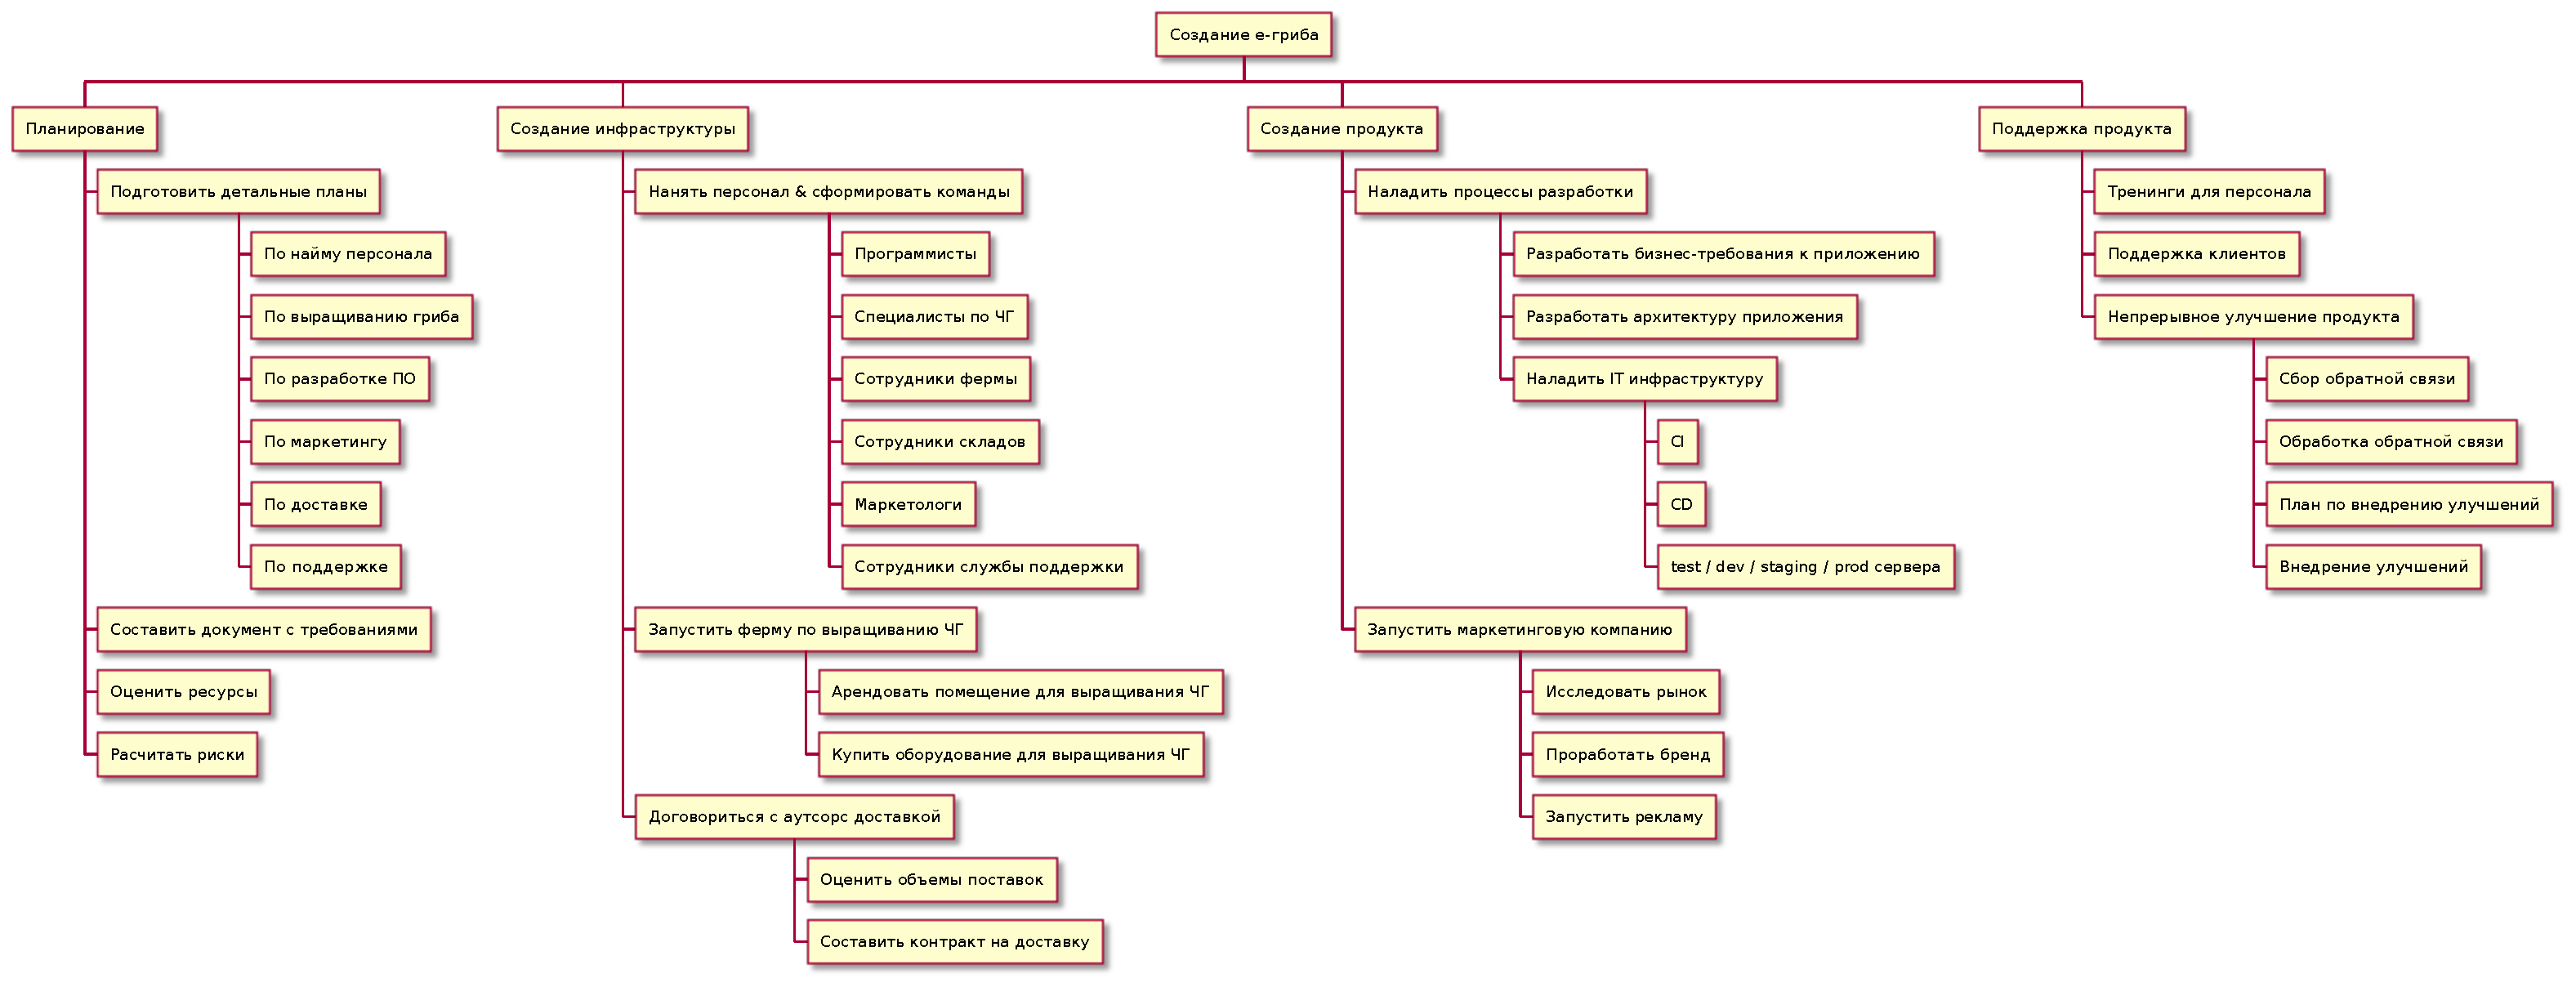
\includegraphics[width=1\textwidth]{./pics/wbs.pdf}
        \centering
    \end{figure}

\section{Оценка проекта}



\subsection{UCP-оценка проекта:}

\subsubsection{UAW}
\begin{itemize}
  \item Server -- 2
  \item Client -- 2
  \item API -- 1
  \item GUI -- 3
  \item DBs -- 2
  \item $UAV =  2 + 2 + 1 + 3 + 2 = 10$
\end{itemize}

\subsubsection{UUCW}
\begin{itemize}
    \item Покупка ЧГ \footnote{Чайный гриб} 4-7
    \item Логин/Регистрация в приложении -- 1-3
    \item Обращение в поддержку -- 1-3
    \item Получение информации о ЧГ --  1-3
    \item $UUCW = 3 \times 5 + 10 = 25$
\end{itemize}

\subsubsection{TCF}
\begin{itemize}
    \item Распределенная система -- 1
\item Время отклика/цели производительности  -- 5
\item Эффективность конечного пользователя -- 3
\item Внутренняя сложность обработки -- 2
\item Переиспользование кода -- 1 
\item Простота установки -- 5
\item Простота использования -- 5
\item Переносимость на другие платформы -- 3
\item Техническое обслуживание -- 5
\item Параллельная обработка  -- 1
\item Безопасность -- 2
\item Доступ к сторонним приложениям  -- 5
\item Обучение пользователей -- 3
\item $SUM = 1\times2.0 + 5\times1.0 + 3\times1.0 + 2\times1.0 + 1\times1.0 + 5\times0.5 + 5\times0.5 + 3\times2.0 + 5\times1.0 + 1\times1.0 + 2\times1.0 + 5\times1.0 + 3\times1.0 = 37$
\item $TCF =  0.6 + \frac{37}{100} = 0.97$
\end{itemize}

\subsubsection{ECF}
    \begin{itemize}
    \item Знакомство с используемым процессом разработки -- 2
    \item Опыт использования приложения -- 1
    \item Объектно-ориентированный опыт команды -- 5
    \item Возможности ведущего аналитика -- 4
    \item Мотивация команды -- 3
    \item Стабильность требований -- 3
    \item Частичная занятость -- 2
    \item Сложность ЯП -- 1
    \item $SUM = 2 \times 1.5 + 1\times0.5 + 5\times1.0 + 4\times0.5 + 3\times1.0 + 3\times2.0 + 2\times(-1) + 1\times(-1) = 16.5$
    \item $ECF = 1.4 + (-0.03 \times 16.5) = 0.905$
\end{itemize}

\subsubsection{Итого}


    \begin{itemize}
        \item $UCP = (UAW + UUCW) \times TCF \times ECF = (10 + 25) \times 0.97 \times (0.905) = 30.72$
        \item Затраты = $UCP \times 30 = 921.6$ человеко-часов
        \item Стоимость проекта = $921.6 \times 2000 \times 1.5 = 2.8$ млн. руб.;
        \item Штат сотрудников (программистов) -- 5
        \item $\frac{921.6}{5 \times 8} = 23$ дня
    \end{itemize}

\subsection{Экспертная оценка}

    Исходя из полученных результатов UCP-оценки проекта, можно сделать вывод, что бюджет и сроки проекта поставлены корректно: 5 программистов будут разрабатывать ПО проекта в течение 23 дней, что удовлетворяет бюджету и срокам.

    На разработку ПО выделено 3 млн. рублей, что является правильным решением, поскольку большая часть бюджета должна быть потрачена на выращивание ЧГ, поддержку, рекламную компанию. Важным моментом является то, что UCP оценка произведенная даже до начала выполнения проекта дает весьма точную оценку затрат, вне зависимости от уровня навыков команды разработчиков. Также, так как наш программный комплекс не является очень сложным и программисты нам нужны всего-лишь на один месяц нам надо изначально точно рассчитать требуемое количество, во избежание последующего до найма (как известно по книге Брукса ``Мифический человеко-месяц'' добавление программистов в готовую команду -- путь в никуда). 

    UCP оценка была произведена опытными людьми с учетом всех технических факторов и факторов окружающей среды, что говорит о ее высокой точности. Тем не менее, на ранних этапах жизни проекта допускается ее небольшое изменение.












\section{Условия оплаты}



    \begin{itemize}
        \item Аванс: 1 млн. руб.;
        \item 5 выплат после выполнения вышеописанных стадий в размере 100 тыс. руб.;
        \item Выплата после завершения работ в размере 2.5 млн. руб.
    \end{itemize}



\end{document}
